\section{Implementation}
In this chapter, the aim is to:

\begin{itemize}
    \item Provide a detailed description of the Python code used to estimate cuffless blood pressure from PPG signals
    \item Discuss any changes or justifications made to the code
\end{itemize}

\subsection{Filtering the dataset}
As discussed in Chapter 3, the MIMIC Database includes data
recorded for 72 ICU patients, ranging from patient indexes '037' to '485'. Firstly, it was necessary to check which 
of these patients contained signal data for the PPG and ABP channels. In Python, this was performed by inspecting the 
\texttt{wfdb.rdrecord.sig\_name} string array for each patient record, and checking to see if the ABP and PPG channels were present (indicated by the 
\texttt{ABP} and \texttt{PLETH} keywords). As a result, the following patients were excluded from the dataset:

\begin{itemize}
    \item '037'
    \item '208'
    \item '209'
    \item '210'
    \item '222'
    \item '262'
    \item '291'
    \item '405'
    \item '413'
    \item '415'
    \item '450'
\end{itemize}\noindent Hence, there was now data available from 61 ICU patients.

\subsection{Decision on the window length}
The next stage is to split up the PPG signal into discrete intervals of the same time interval. In order to justify the window length used, 
it was necessary to analysis the waveform structure of the PPG for particular patients, as shown in Figure \ref{windowing}. 

\begin{figure}[H]
    \centering
    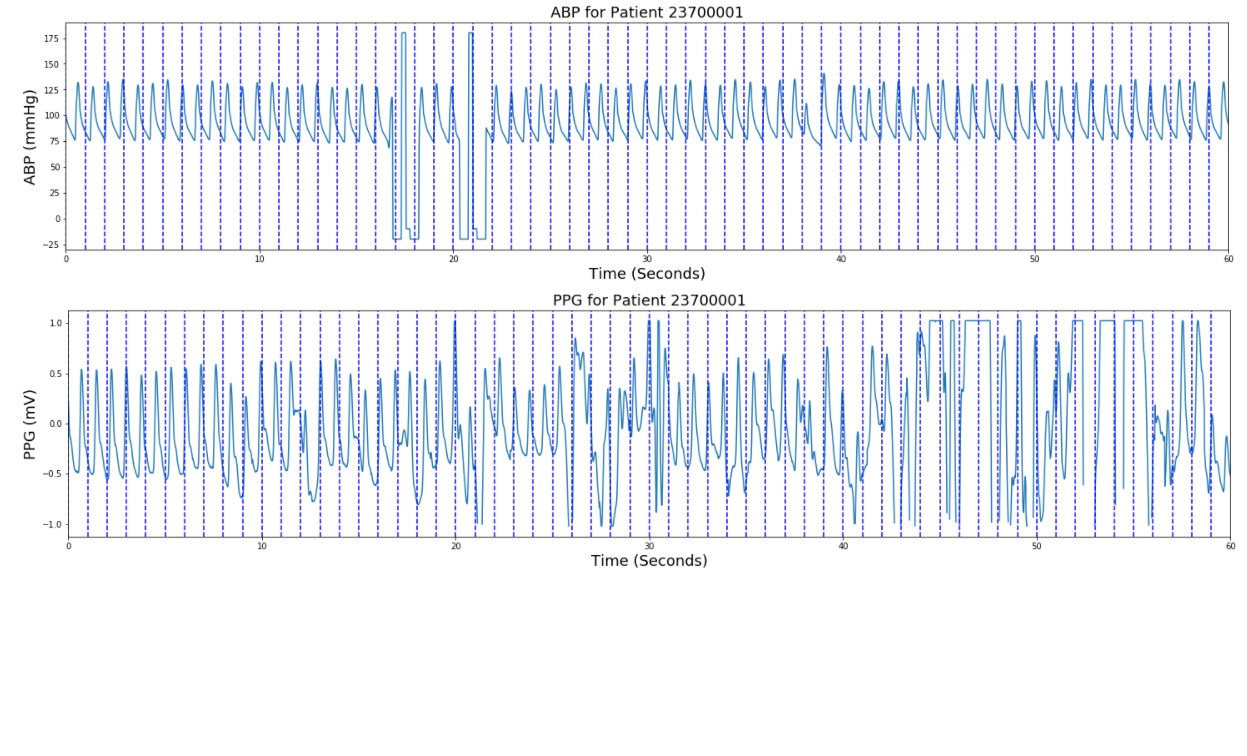
\includegraphics[width=16cm,height=16cm,keepaspectratio]{Implementation/window.png}
    \caption{ABP and PPG signals for patient record 23700001}
    \label{windowing}
\end{figure}\noindent Based on the windowing segments in Figure \ref{windowing}, it was ascertained that 
sufficient physiological information about the PPG signal could be picked up within each window, as there is access to both a maximum and minimum. Hence, 
there would be sufficient PPG features for the neural network models to learn from within each window.



\subsection{Choosing the patients}
Based on the decision to use a window length of 1 second, it was necessary to take a subset of the dataset.  
This was because a small window length implies that a lot of datapoints are available for training already. For example, if there are 1000 seconds worth of data and a window of 10 seconds is applied, then there will be 100 discrete datapoints available for training. Therefore, it is not necessary to acquire data from all 61 patients in the MIMIC database. By considering that the motivation of the FYP is to investigate the detection and prevention 
of hypertension, the decision was to examine the records of patients suffering with 
Cardiovascular diseases or other heart-related illnesses. Hence, a subset of the MIMIC I database was chosen, as illustrated 
in Table \ref{tabDatasetChosen}.
\begin{table}[H]
    \centering
    \caption{Characteristics of the chosen 12 patients from the MIMIC-I database}
    \label{tabDatasetChosen}
    \begin{tabular}{cccc}
    \hline
    \textbf{Patient record number} & \textbf{Age} & \textbf{Gender} & \textbf{Health condition} \\ \hline
    418 & 52 & M & CHF/pulmonary edema  \\
    480 & 52 & M & Post-op CABG         \\
    237 & 63 & F & MI/cardiogenic shock \\
    477 & 67 & M & Post-op CABG         \\
    466 & 70 & M & CHF/pulmonary edema  \\
    476 & 72 & F & Post-op CABG         \\
    225 & 73 & M & CHF/pulmonary edema  \\
    230 & 75 & F & CHF/pulmonary edema  \\
    213 & 82 & F & CHF/pulmonary edema  \\
    212 & 84 & M & CHF/pulmonary edema  \\
    456 & 84 & M & Post-op CABG         \\ 
    417 & 85 & M & CHF/pulmonary edema \\\hline
    \end{tabular}
\end{table}\noindent After processing the data and checking for NaN (not a number) values in the patient recordings, Table \ref{tabSamplesAvailable} 
shows the number of samples available for each patient.

\begin{table}[H]
        \centering
        \caption{Number of samples available after initial preprocessing from the MIMIC database subset}
        \label{tabSamplesAvailable}
        \begin{tabular}{cc}
        \hline
        \textbf{Patient record number} & \textbf{10-minute Samples} \\ \hline
        418 &  0\\
        480 &  30\\
        237 &  17\\
        477 &  3\\
        466 &  139\\
        476 &  67\\
        225 &  17\\
        230 &  38\\
        213 &  42\\
        212 &  143\\
        456 &  83\\
        417 &  0\\ \hline
        \end{tabular}
\end{table}   

\subsection{Extracting the ground truth blood pressure values}
Before the ground truth blood pressure values are extracted from the ABP signals, the following sanity checks are applied:
\begin{itemize}
    \item Check that the calculated Systolic peaks are within the range of $60-210 mmHg$. An additional threshold of $30 mmHg$ to the most extreme blood pressure values in Table \ref{bp_vals_table} has been applied to account for the most serious cardiac patients
    \item Check that the calculated Diastolic peaks are within the range $30-140 mmHg$. The same threshold has been applied here as well
    \item The Normal-to-Normal (NN) interval and Heart Rate (HR) are calculated for each particular window.
    \item If the NN interval is not a reasonable value (within the range of 0.3 to 1.4 seconds) then the value is discarded
    \item If the heart rate is not a reasonable value (within the range of 50 to 140 Beats per minute), then the value is discarded
    \item Both the Systolic and Diastolic peaks are checked for NaNs (not a number) values
    \item Finally, within each signal window, the ground truth blood pressure value is taken as the median of all blood pressure values found in that particular window
\end{itemize}


\subsection{Preprocessing the PPG signal}
The $Z$-score normalisation equation is applied to the PPG signal, 
\begin{equation}
    Z_{i} = \frac{(PPG_{i} - \mu_{PPG_i}) }{\sigma_{PPG_i}}
\end{equation} \noindent where $Z_{i}$ is the $Z$-score normalised PPG signal for a particular window $i$, 
$PPG_{i}$ is the raw PPG signal, $\mu$ is the mean of the PPG signal and $\sigma$ is the standard deviation. $Z$-score 
normalisation was used instead of minimum-maximum (min-max) normalisation, as this method is less affected by outliers in the data. In addition, a 4th order 
Butterworth bandpass filter with cutoff frequencies of 0.5 and 40 Hz respectively are applied to the PPG. This is applied based on what was discussed 
in a previous implementation discussed in the literature review \cite{Nath2018}. The filter is used to 
remove both low frequency noise and baseline wander from the signal. These operations are performed using the following Python code,
\begin{figure}[H]
    \begin{python}
import numpy as np
from scipy.signal import butter, filtfilt
# 4th order butterworth filter for PPG preprocessing
b,a = butter(4,[0.5, 40], 'bandpass', fs=fs)   

for i in range(0, NumberWindows):
    ppg_win = filtfilt(b,a, ppg_win)
    ppg_win = ppg_win - np.mean(ppg_win)
    ppg_win = ppg_win/np.std(ppg_win)
    ppg_record[i, :] = ppg_win
    \end{python}
    \caption{Python code for the preprocessing of the PPG signal}
\end{figure}


\subsection{Processing of data before training}
After the PPG signals of the MIMIC database subset have been preprocessed and segmented with 1-second windows, there are now $337998$ PPG samples available in total for training with the neural network models. 
The data is split into training, testing and validation sets in the ratio of 50:25:25. It is also ensured in the Python code created that training is only performed on the data of 1 subject at any time. 
This is extremely important because as discussed previously, the subjects are not the same in gender, age and have different cardiovascular diseases. Hence, the data is now ready to be 
learned on by the proposed neural network models. Hence, the distributions of the ground truth Systolic and Diastolic blood pressure values for the three 
datasets can be displayed for the training set in Figures \ref{histSBP} and \ref{histDBP}.
\begin{figure}[H]
    \centering
    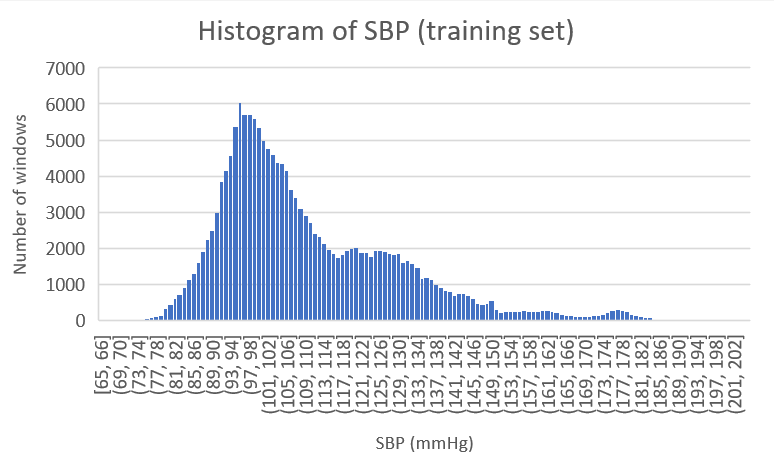
\includegraphics[width=15cm,height=15cm,keepaspectratio]{Implementation/trainingSbp.png}
    \caption{Histogram of the SBP ground truth values in the training set}
    \label{histSBP}
\end{figure}
\begin{figure}[H]
    \centering
    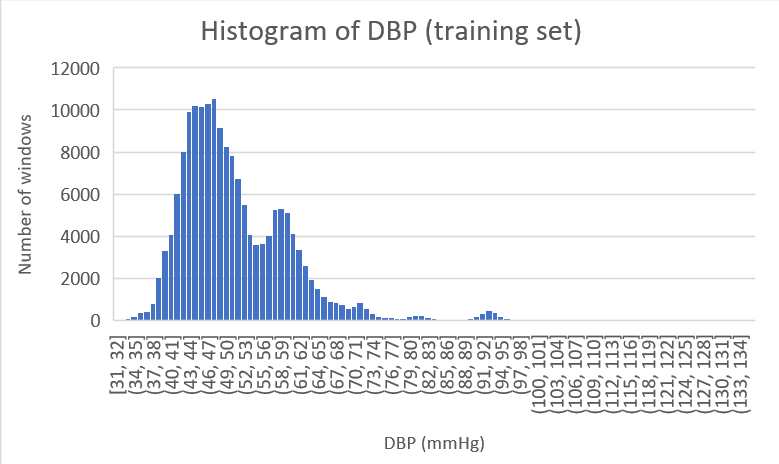
\includegraphics[width=15cm,height=15cm,keepaspectratio]{Implementation/trainingDbp.png}
    \caption{Histogram of the DBP ground truth values in the training set}
    \label{histDBP}
\end{figure}\noindent The histograms of the SBP and DBP for the testing and validation 
sets also have a similar distribution to the training set, and hence are not included in this report.

\subsection{Overview of Neural Network models used}
In this section, a breakdown of the five proposed neural network models for experimentation, stated previously in Chapter 3, are discussed.
\subsubsection{CNN AlexNet model}
An overview of the AlexNet architecture \cite{alexNet} used for this FYP is demonstrated in Figure \ref{alexnetArch} (using the terminology from the Python Keras documentation). 
\begin{figure}[H]
    \centering
    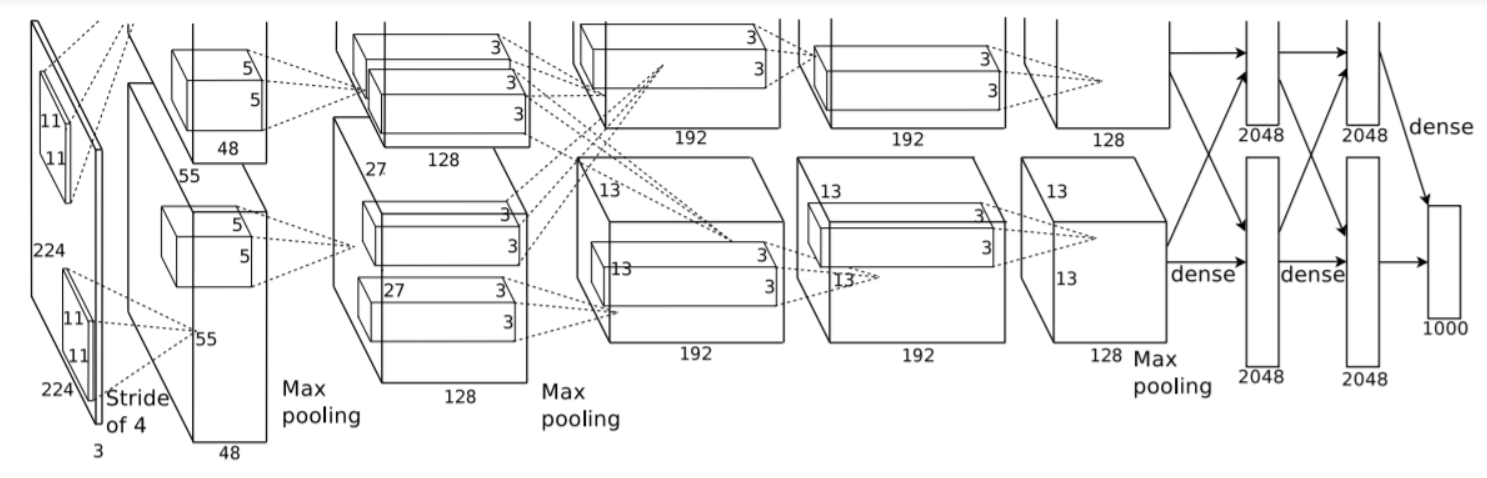
\includegraphics[width=15cm,height=15cm,keepaspectratio]{Implementation/alexnetArch.png}
    \caption{Overview of the AlexNet architecture}
    \label{alexnetArch}
\end{figure}\noindent The following comments are made about the components of this architecture:
\begin{itemize}
\item PPG' and PPG'' refer to the first and second derivatives of the PPG signal with respect to time. This is implemented using the following Python code,
\begin{figure}[H]
    \begin{python}
        import tensorflow as tf
        # data_in_shape = size of windowed PPG segment
        # Input function is the input layer to the neural network model
        X_input = Input(shape=data_in_shape)
        # sampling frequency        
        fs = 125
        # first derivative calculation                                    
        dt1 = (X_input[:,1:] - X_input[:,:-1])*fs
        # second derivative calculation   
        dt2 = (dt1[:,1:] - dt1[:,:-1])*fs           
        dt1 = tf.pad(dt1, tf.constant([[0,0],[0,1],[0,0]]))
        dt2 = tf.pad(dt2, tf.constant([[0,0],[0,2],[0,0]]))
        X = tf.concat([X_input, dt1, dt2], axis=2)
        
        \end{python}    
        \caption{Feature extraction of PPG first and second temporal derivatives}
    \label{pythonDeriv} 
\end{figure}
    \item In Figure \ref{pythonDeriv}, the first derivative is found by first calculating the difference between the input data and the input data with a delay of 1 sample. This difference is then multiplied by the PPG sampling frequency, $f_s = 125 Hz$, as this can be effectively expressed as the rate of how many samples are processed in 1 second. This is mathematically expressed as,
    \begin{align}
        PPG' &= \bigg(x_{PPG}(t + 1) - x_{PPG}(t)\bigg) \times f_s = \frac{d}{dt} \bigg(x_{PPG}(t + 1) - x_{PPG}(t)\bigg)\\
        \therefore PPG' &= PPG' \times f_s = \frac{d}{dt} (PPG')
    \end{align}\noindent In addition, a further multiplication of the first derivative by the sampling frequency produces a result for the second derivative, $PPG''$, as illustrated above. This code is applied directly to the four other proposed neural network architectures
    \item Conv1D(96, kernel size = 7, stride = 3) is a 1-dimensional convolutional layer with 96 filters. Kernel size specifies the size of the 1-dimensional convolutional window applied to the data. A stride of 3 means that the convolutional window will move 3 units at a time
    \item MaxPooling1D(3, stride = 3) is a 1-dimensional maximum pooling layer with a window size of 3. This layer takes the maximum value within each set window
    \item The ReLU activation function has been discussed previously in Chapter 2
    \item Batch Normalisation transforms the input data such that the average output is approximately 0 and the standard deviation is approximately 1
    \item The Flatten layer flattens the input data into a 1-dimensional vector
    \item The Dense layer (4096) is a fully connected layer which produces an output vector of size 4096
    \item The Dropout layer is used to prevent overfitting. The Dropout layer randomly sets a fraction of the input units to 0 (in this case 0.5)
    \item The Systolic and Diastolic blood pressure estimates are returned through a Dense layer with an output vector dimensionality of 1
\end{itemize}

\subsubsection{CNN ResNet model}
The architecture of the ResNet model is directly based on the 34-layer residual architecture described in the paper \emph{Deep Residual Learning for Image Recognition} \cite{resnetArch}, and is illustrated in Figure \ref{resnetArc}.
\begin{figure}[H]
    \centering
    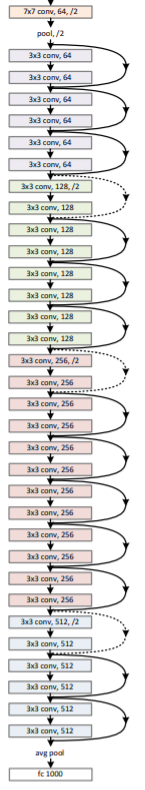
\includegraphics[width=16cm,height=16cm,keepaspectratio]{Implementation/resnetArch.png}
    \caption{Overview of the ResNet architecture}
    \label{resnetArc}
\end{figure}\noindent The input is also modified to include a feature extraction stage for $PPG'$ and $PPG''$ as discussed previously.

\subsubsection{ResNet with Leave One Subject Out (LOSO) model}
The architecture of the ResNet with LOSO model was proposed in the paper \emph{Blood Pressure Estimation from Photoplethysmogram Using a Spectro-Temporal Deep Neural Network} \cite{slapnicar2019}. This architecture is classified as 
a spectro-temporal neural network, as it utilises features of the signal in both the time and frequency domains. 
\begin{figure}[H]
    \centering
    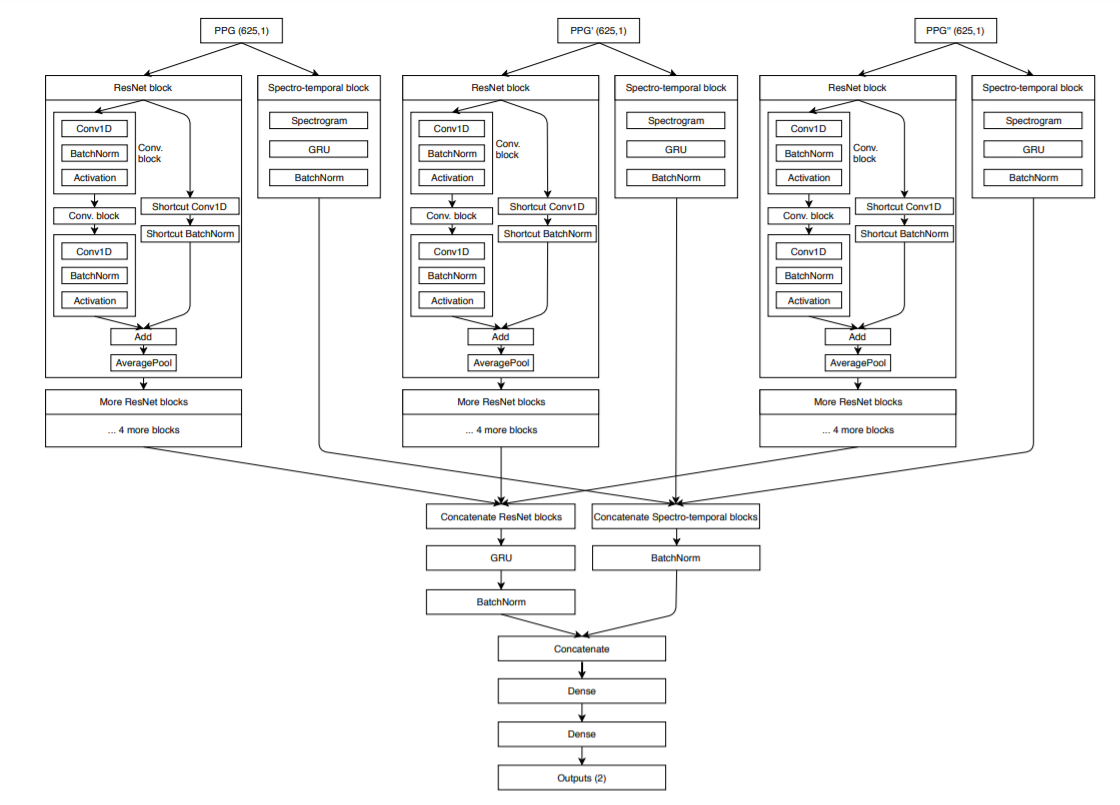
\includegraphics[width=16cm,height=16cm,keepaspectratio]{Implementation/slapnicar.png}
    \caption{Overview of the ResNet-LOSO architecture \cite{slapnicar2019}}
    \label{slapnicarArch}
\end{figure}\noindent The following comments are made about the components of this architecture:
\begin{itemize}
    \item The term LOSO refers to how the experiment was conducted in the original paper. LOSO is a cross-validation technique where the dataset is split according to the number of subjects available. In addition to this, one subject is randomly selected for testing the model and the other subjects are used to train the model. This is repeated until all the subjects have been used for the test dataset.
    \item As indicated in Figure \ref{slapnicarArch}, the architecture consists of three distinct blocks, with the difference being what the blocks take as input. The three blocks take the windowed PPG, the first derivative and the second derivative of the PPG signal with respect to time
\end{itemize}


\subsubsection{LSTM model}
The Bi-directional LSTM model architecture used for experimentation in this FYP is illustrated in Figure \ref{lstmArch}.
\begin{figure}[H]
    \centering
    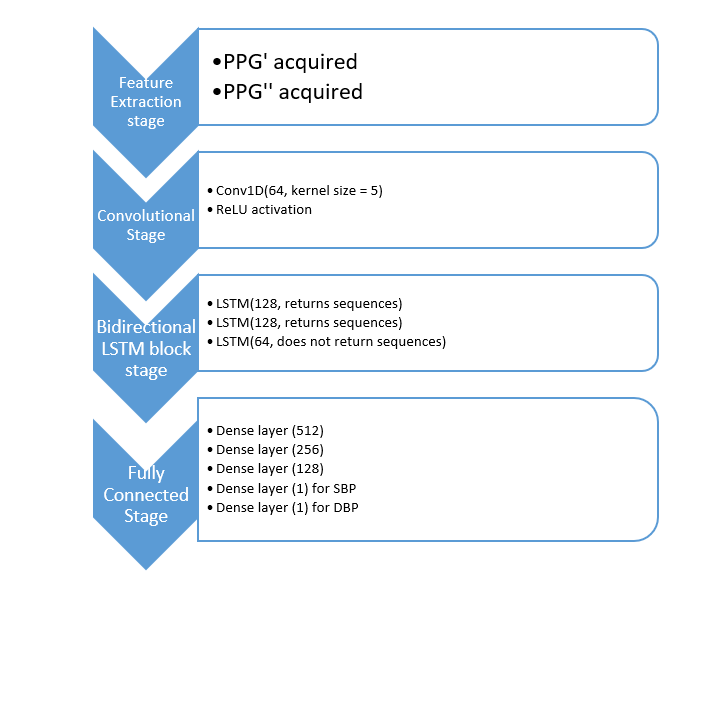
\includegraphics[width=16cm,height=16cm,keepaspectratio]{Implementation/lstmArch.png}
    \caption{Overview of the Bi-directional LSTM architecture}
    \label{lstmArch}
\end{figure}\noindent The following comments are made about the components of this architecture:
\begin{itemize}
    \item LSTM(128) creates an LSTM layer with 128 units
    \item When the LSTM layer returns sequences, the layer outputs the full sequence of hidden states, $[h_1, h_2, \dots, h_n]$. Otherwise, only the last hidden state, $h_n$ is returned as the output of the layer 
\end{itemize}


\subsubsection{Proposed Transformer Encoder model}
The Transformer Encoder model architecture used for experimentation in this FYP is illustrated in Figure \ref{lstmArch}.
\begin{figure}[H]
    \centering
    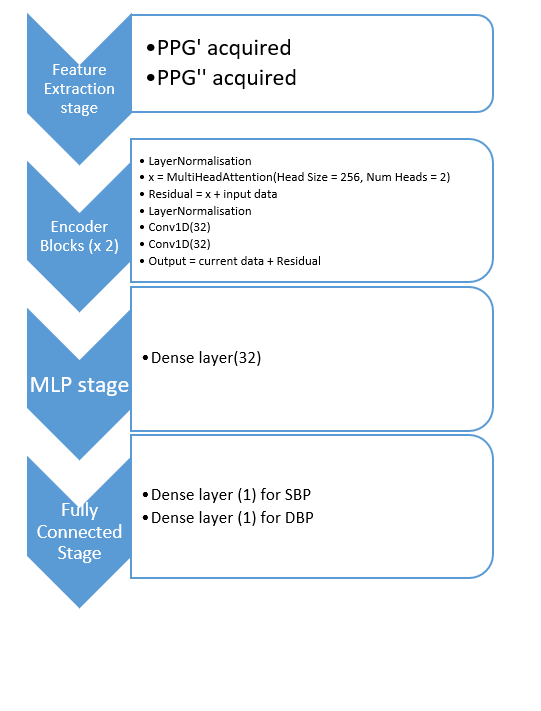
\includegraphics[width=16cm,height=16cm,keepaspectratio]{Implementation/transformerArch.png}
    \caption{Overview of the Transformer Encoder architecture}
    \label{transformerArch}
\end{figure}\noindent The following comments are made about the components of this architecture:
\begin{itemize}
    \item The architecture has the following parameters available that can be changed:
    \begin{itemize}
        \item The number of encoder blocks
        \item The head size in the encoder block
        \item The number of heads in the encoder block
        \item The number of filters in the Conv1D layers in the encoder block
        \item The number of Multi Layer Perceptron (MLP) units
    \end{itemize}
    \item For this FYP, these parameters have been chosen in order to address the tradeoff between minimizing the training time of the model whilst aiming to maximising the accuracy of the cuffless estimation of blood pressure values
\end{itemize}\noindent To conclude this chapter, an overview has been given of the five neural network architectures used for the cuffless estimation of blood pressure values. The specific layers and parameters used in the Python code have 
also been highlighted for further understanding as to how the architectures differ from each other. Hence, it is now suitable to proceed with the testing plan in the next chapter.